\documentclass{beamer}

\let\val\undefined
\usepackage{pgf}
\usepackage{pgfplots}
\usepackage{tikz}
\usepackage{booktabs}
\usepackage{natbib}
\usepackage{algorithm2e}
\usepackage{siunitx}
\usepackage{framed}
\usepackage{longtable}
\usepackage{amsmath}
\usepackage{amsthm}
\usepackage{bigdelim,multirow}
\usepackage{grffile}

\usetheme[progressbar=frametitle]{metropolis}
\usepackage{libertine}

\usetikzlibrary{arrows,automata,backgrounds,positioning,decorations,intersections,matrix}

% *** Styles ***
%\setbeamertemplate{navigation symbols}{}
\usecolortheme{dolphin}
%\usecolortheme{rose}
\setbeamercovered{transparent}
\usefonttheme{professionalfonts}
%\usefonttheme[onlymath]{serif}

% *** Colors ***
\newcommand{\tc}[2]{\textcolor{#1}{#2}}
\newcommand{\tcb}[1]{\tc{blue}{#1}}
\newcommand{\tcr}[1]{\tc{red}{#1}}
\newcommand{\tcg}[1]{\tc{green}{#1}}

\def\checkmark{\tikz\fill[scale=0.4](0,.35) -- (.25,0) -- (1,.7) -- (.25,.15) -- cycle;}

\newcommand{\Ex}{\mathbb{E}}
%\newcommand{\Pr}{\mathbb{P}}
\DeclareMathOperator{\Var}{Var}

\definecolor{varcolor}{RGB}{132,23,49}
\newcommand{\varname}[1]{\textcolor{varcolor}{\mathsf{#1}}}

\title{Introduction to Machine Learning}
\author{Samuel Carton (adapted from Marek Petrik)}
\date{8/2025}

\begin{document}
	\begin{frame}
		\maketitle
		\tiny{Some of the figures in these slides are taken from "An Introduction to Statistical Learning, with applications in R"  (Springer, 2013, 2021) with permission from the authors: G. James, D. Witten,  T. Hastie and R. Tibshirani }

\end{frame}

\begin{frame} \frametitle{What is machine learning?}
    Arthur Samuel (1959, IBM, computer checkers):
    \begin{quote}
Field of study that gives computers the ability to learn without being explicitly programmed
    \end{quote}

    \begin{center}
        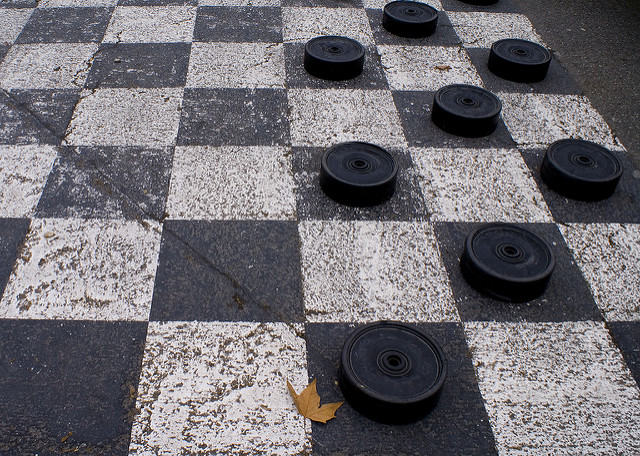
\includegraphics[width=0.6\linewidth]{../figs/class1/checkers.jpg}\\
        {\tiny Creative commons license, Source: \url{http://flickr.com}}
    \end{center}
\end{frame}

\begin{frame} \frametitle{IBM Watson: Computers Beat Humans in Jeopardy}
    \centering
    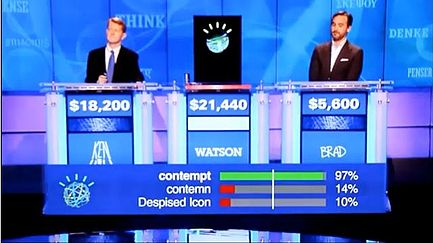
\includegraphics[width=0.8\linewidth]{../figs/class1/Watson_Jeopardy.jpg} \\
    \tiny{Fair use, \url{https://en.wikipedia.org/w/index.php?curid=31142331}}
\end{frame}

%	\begin{frame} \frametitle{AlphaGo: Computers Beat Humans in Go}
%		\centering
%		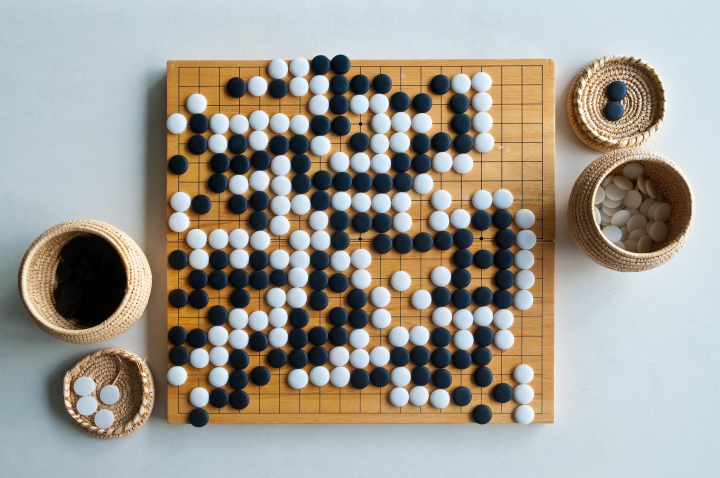
\includegraphics[width=0.8\linewidth]{../figs/class1/go_image.jpg} \\
%		\tiny{Photograph by Saran Poroong — Getty Images/iStockphoto }
%	\end{frame}

\begin{frame} \frametitle{AlphaFold: Machine Learning for Protein Folding}
\centering
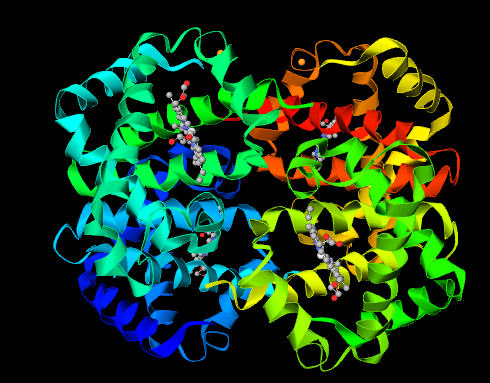
\includegraphics[width=0.8\linewidth]{../figs/class1/alphafold.png} \\
\end{frame}

\begin{frame}{Predicting Elections}
\centering
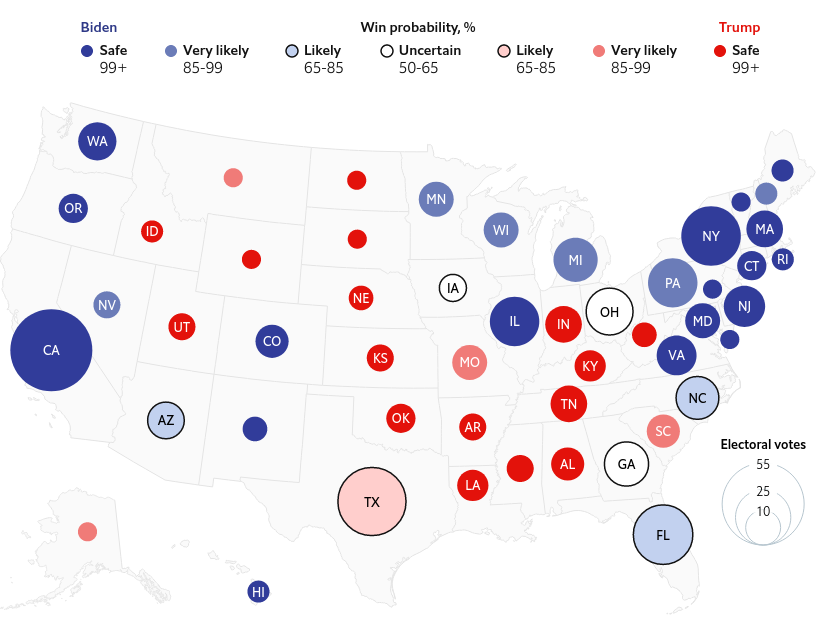
\includegraphics[width=0.8\linewidth]{../figs/class1/elections.png} \\
\tiny{\url{https://economist.com}}
\end{frame}

\begin{frame} \frametitle{Personalized Product Recommendations}
    \centering
    Online retailers mine purchase history to make recommendations\\ [3mm]
    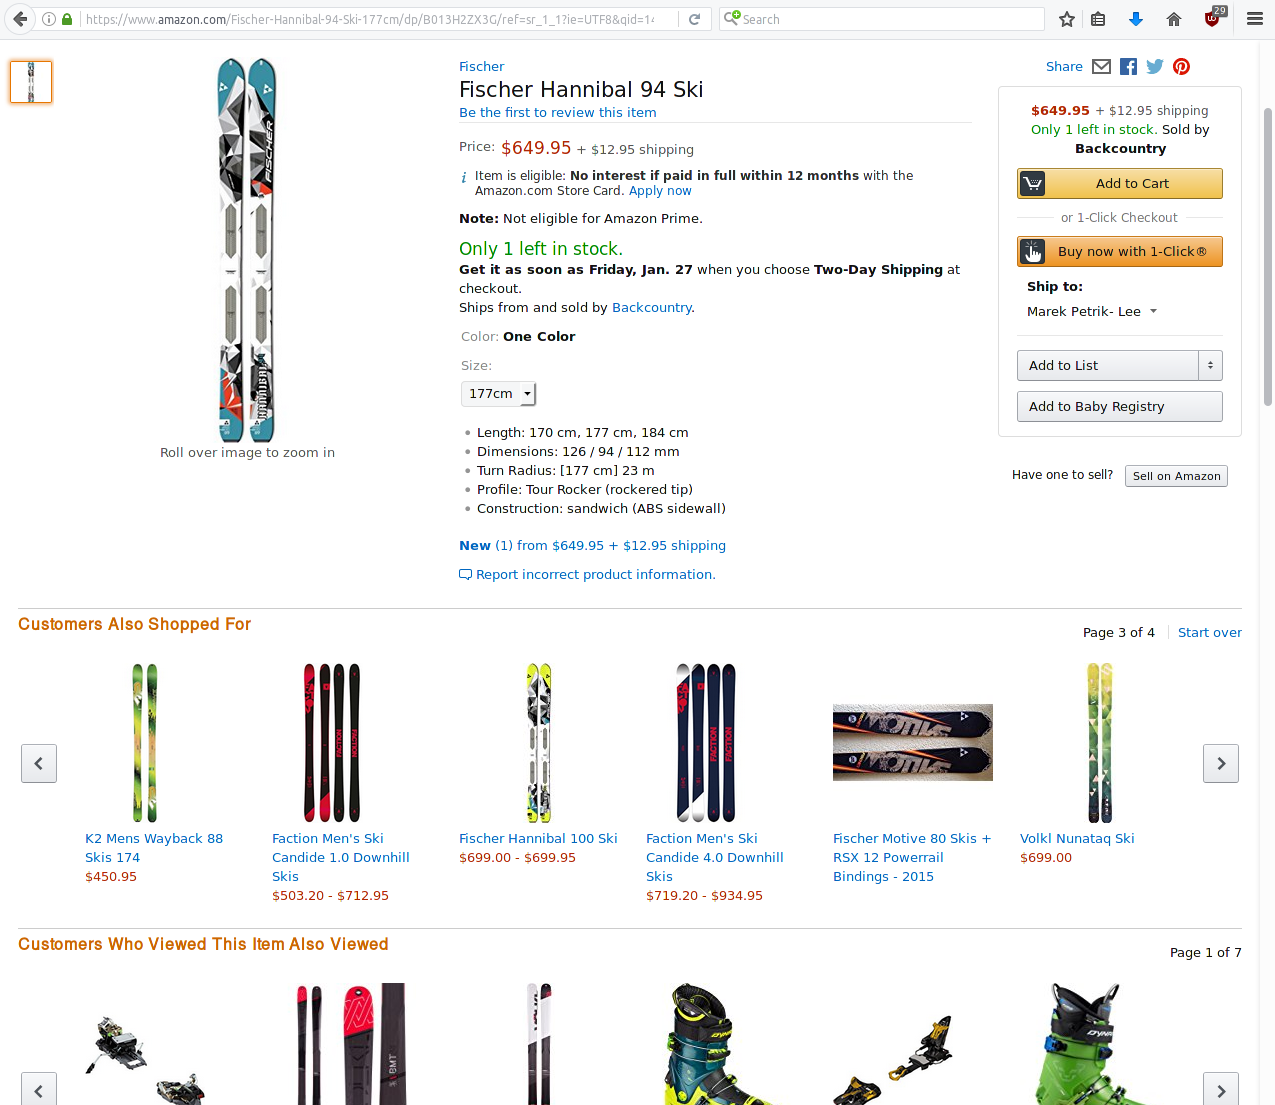
\includegraphics[width=0.7\linewidth]{../figs/class1/recommendation.png}
\end{frame}


\begin{frame} \frametitle{Predicting Strength of Hurricanes}
    \centering
    \emph{NOAA Models}: \texttt{SHIFOR,SHIPS,DSHIPS,LGEM} \\ [3mm]
    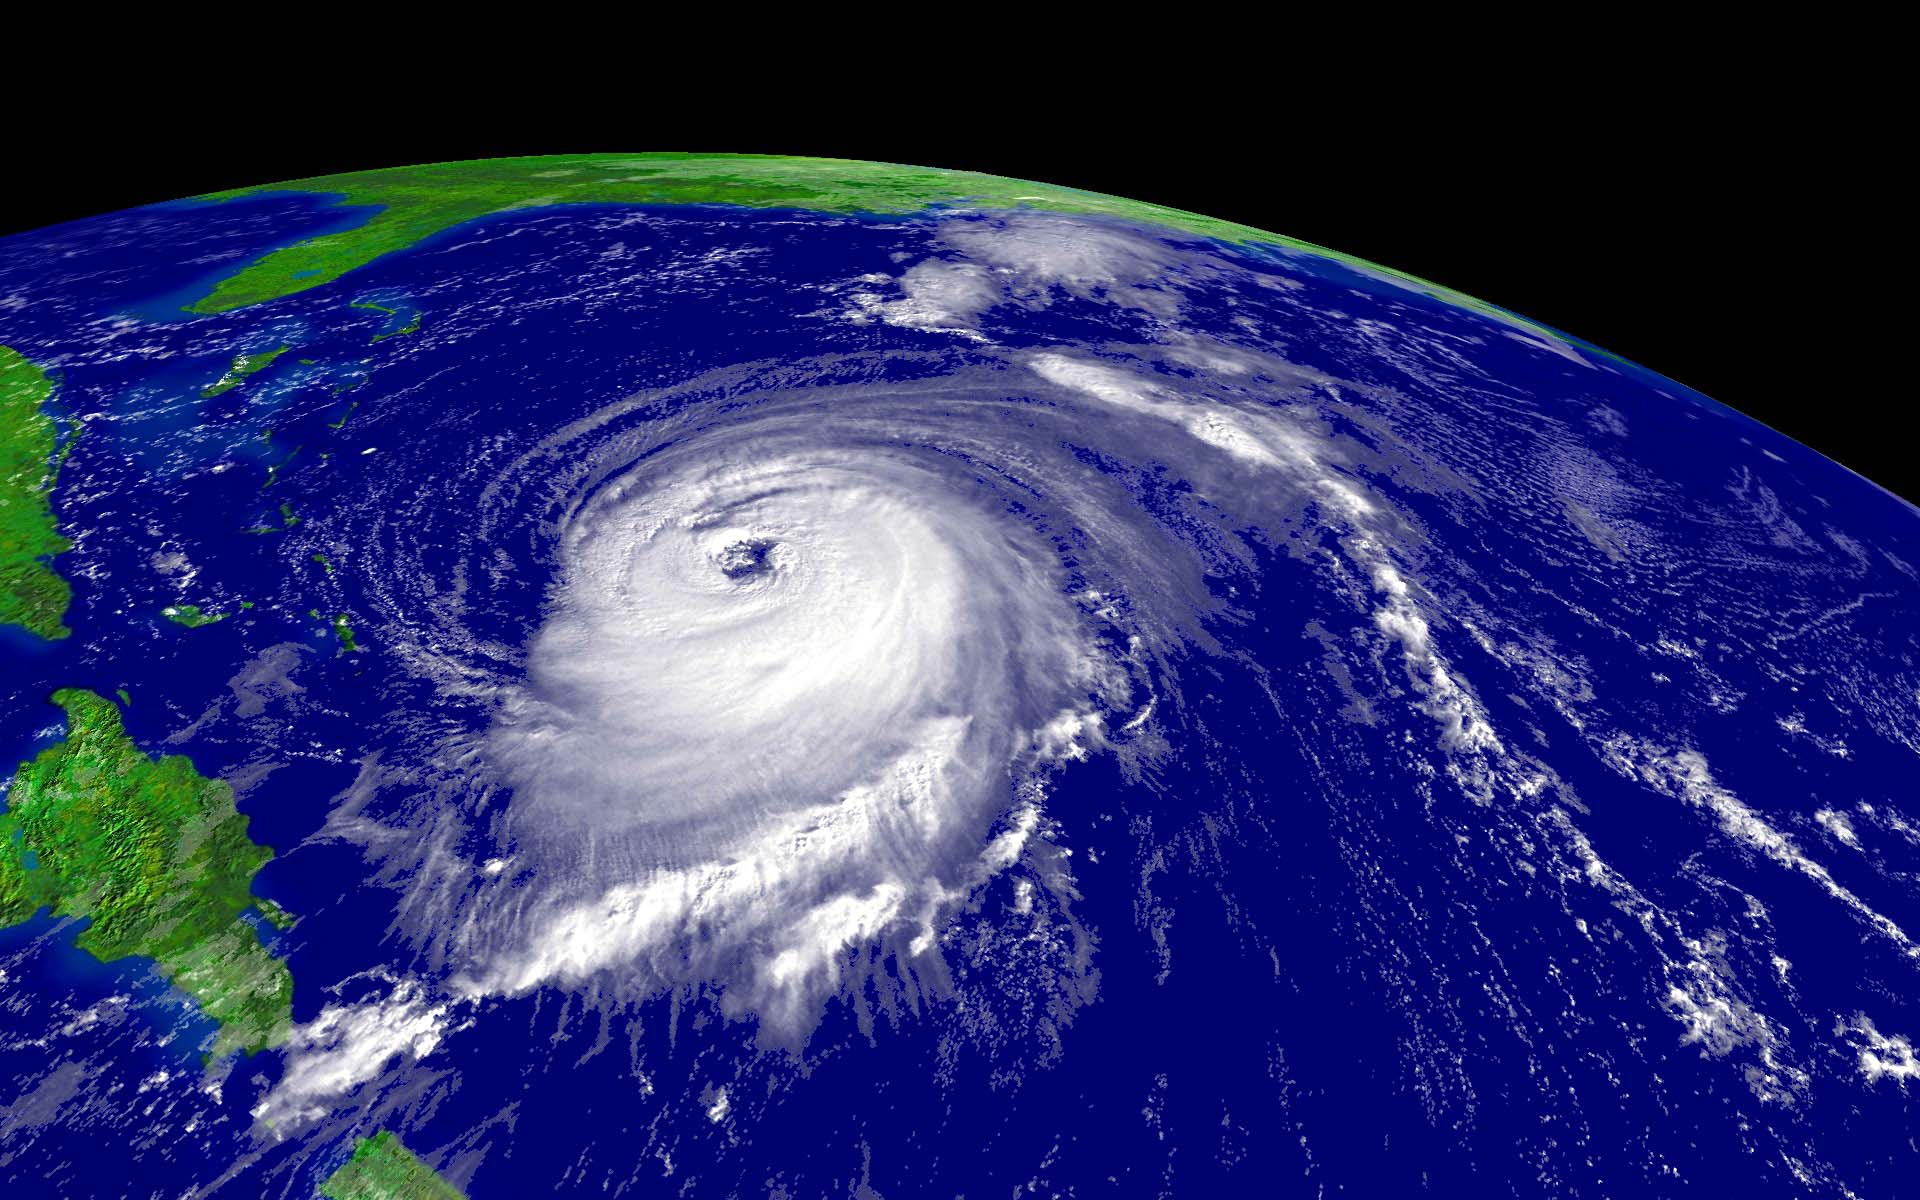
\includegraphics[width=0.8\linewidth]{../figs/class1/hurricane_image.jpg} \\
    \tiny{Hurricane Isabel, 2003, Source: NOAA.gov }
\end{frame}

\begin{frame} \frametitle{Other Applications}
    \begin{enumerate}
            \item Health-care: Identify risks of getting a disease
            \item Detect spam in emails
            \item Recognize hand-written text
            \item Create a fake video (\url{https://www.youtube.com/watch?v=cQ54GDm1eL0})
    \end{enumerate}

    \alert{Any other applications?}
\end{frame}


\begin{frame} \frametitle{What is Machine Learning}
    \begin{itemize}
            \item Discover unknown function $\alert{f}$:
            \[ \tcb{Y} = \tcr{f}(\tcg{X})  \]
            \item $\tcr{f}$ = \textbf{hypothesis}, or model
            \item $\tcg{X}$ = \textbf{features}, or predictors, or inputs
            \item $\tcb{Y}$ = \textbf{response}, or target
    \end{itemize}
    \[ \varname{MPG} = \alert{f}(\varname{Horsepower}) \]
    \begin{center}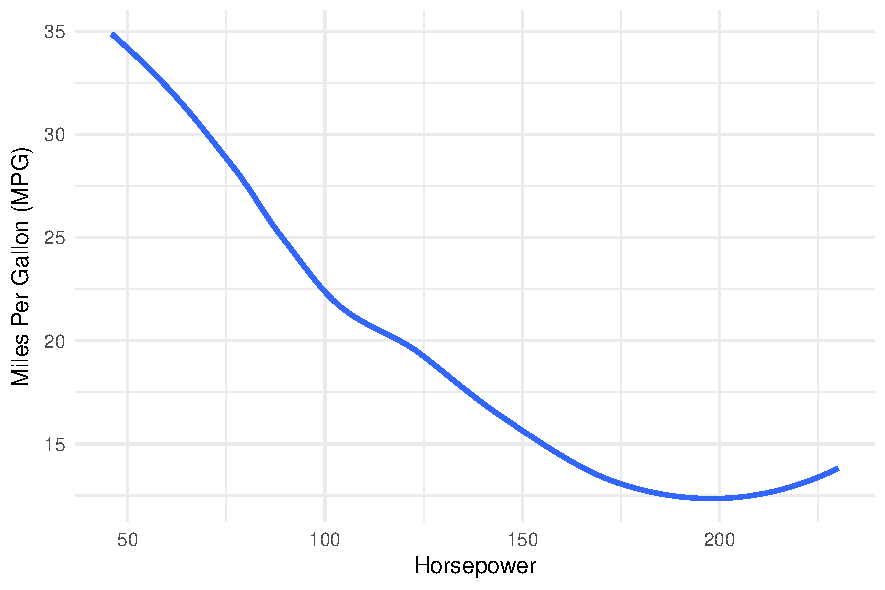
\includegraphics[width=0.5\linewidth]{../figs/class1/auto_function.pdf}\end{center}
\end{frame}

\begin{frame} \frametitle{Machine Learning}
\centering
    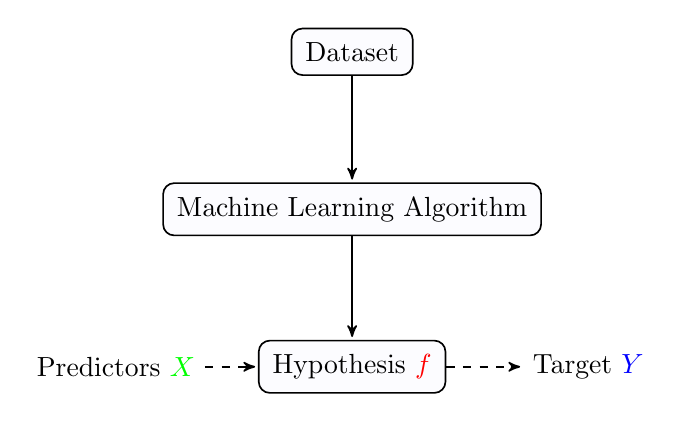
\begin{tikzpicture}[->,>=stealth',shorten >=1pt,auto,node distance=2cm,semithick,block/.style = {rounded corners, draw,fill=blue!1,align=center,inner sep=5}]
            \node[block](data){Dataset};
            \node[block,below of=data](algo){Machine Learning Algorithm};
            \node[block,below of=algo](hypo){Hypothesis $\tcr{f}$};
            \node[left of=hypo,xshift=-1cm](input) {Predictors $\tcg{X}$};
            \node[right of=hypo,xshift=1cm](output) {Target $\tcb{Y}$};
            \path (data) edge (algo)
                        (algo) edge (hypo)
                        (input) edge [dashed] (hypo)
                        (hypo) edge [dashed] (output);
    \end{tikzpicture}
    \vfill
    Purpose: Inference or prediction
\end{frame}

\begin{frame} \frametitle{Auto Dataset}
    \centering
    \begin{tabular}{rrrl}
            \hline
            & \tcb{mpg} & \tcg{horsepower} & name \\
            \hline
            1 & 18.00 & 130.00 & chevrolet chevelle malibu \\
            2 & 15.00 & 165.00 & buick skylark 320 \\
            3 & 18.00 & 150.00 & plymouth satellite \\
            4 & 16.00 & 150.00 & amc rebel sst \\
            5 & 17.00 & 140.00 & ford torino \\
            6 & 15.00 & 198.00 & ford galaxie 500 \\
            7 & 14.00 & 220.00 & chevrolet impala \\
            8 & 14.00 & 215.00 & plymouth fury iii \\
            9 & 14.00 & 225.00 & pontiac catalina \\
            10 & 15.00 & 190.00 & amc ambassador dpl \\
            & $\cdots$ & $\cdots$ & $\cdots$ \\
            \hline
    \end{tabular}
\end{frame}

\begin{frame} \frametitle{Auto Dataset}
    \centering
    \begin{center}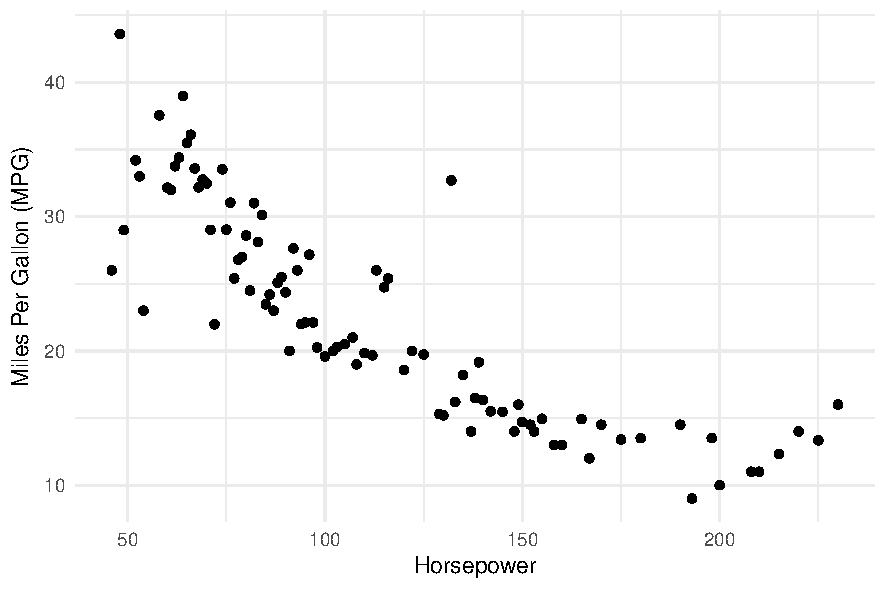
\includegraphics[width=0.9\linewidth]{../figs/class1/auto_data.pdf}\end{center}
\end{frame}

\begin{frame} \frametitle{Bayes Classifier}
    \alert{What is the \tcb{MPG} of a car with \tcg{horsepower} = 150?} \\
    \begin{center}
            \begin{tabular}{rrrl}
            \hline
            & \tcb{mpg} & \tcg{horsepower} & name \\
            \hline
            1 & 18.00 & 130.00 & chevrolet chevelle malibu \\
            2 & 15.00 & 165.00 & buick skylark 320 \\
            3 & 18.00 & 150.00 & plymouth satellite \\
            4 & 16.00 & 150.00 & amc rebel sst \\
            5 & 17.00 & 140.00 & ford torino \\
            6 & 15.00 & 198.00 & ford galaxie 500 \\
            7 & 14.00 & 220.00 & chevrolet impala \\
            8 & 14.00 & 215.00 & plymouth fury iii \\
            9 & 14.00 & 225.00 & pontiac catalina \\
            10 & 15.00 & 190.00 & amc ambassador dpl \\
            \hline
            \end{tabular}
    \end{center}
    \pause
    \[f(x) = \Ex [Y \mid X = x] \]
    \pause
    \begin{itemize}
            \item Achieves the minimum possible error with infinite data
            \item \alert{What if data is finite?}
    \end{itemize}
\end{frame}

\begin{frame} \frametitle{Limitation of Bayes Classifier}
    \alert{What is the \tcb{MPG} of a car with \tcg{horsepower} = 200?} \\
    \begin{center}
            \begin{tabular}{rrrl}
                    \hline
                    & \tcb{mpg} & \tcg{horsepower} & name \\
                    \hline
                    1 & 18.00 & 130.00 & chevrolet chevelle malibu \\
                    2 & 15.00 & 165.00 & buick skylark 320 \\
                    3 & 18.00 & 150.00 & plymouth satellite \\
                    4 & 16.00 & 150.00 & amc rebel sst \\
                    5 & 17.00 & 140.00 & ford torino \\
                    6 & 15.00 & 198.00 & ford galaxie 500 \\
                    7 & 14.00 & 220.00 & chevrolet impala \\
                    8 & 14.00 & 215.00 & plymouth fury iii \\
                    9 & 14.00 & 225.00 & pontiac catalina \\
                    10 & 15.00 & 190.00 & amc ambassador dpl \\
                    \hline
            \end{tabular}
    \end{center}
    \visible<2>{Return the \textbf{nearest neighbor}.}
\end{frame}

\begin{frame} \frametitle{Nearest Neighbor Hypothesis}
\begin{center}
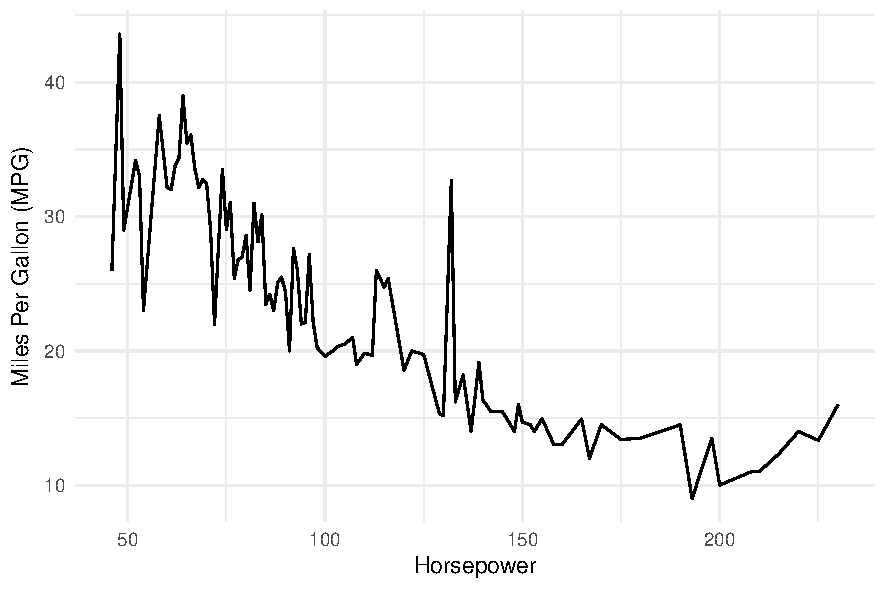
\includegraphics[width=\linewidth]{../figs/class1/auto_data_mean.pdf}
\end{center}
\end{frame}

\begin{frame} \frametitle{Errors in Machine Learning}
    Must allow for errors $\epsilon$:
    \[ \tcb{Y} = \tcr{f}(\tcg{X}) + \epsilon \]
    \pause
    \begin{enumerate}
    \item World is too complex to model precisely
    \item Many features are not captured in data sets
    \item Datasets are limited
    \end{enumerate}

    \begin{center}
            \visible<2>{\alert{How to reduce prediction errors?}}
    \end{center}
\end{frame}

\begin{frame} \frametitle{KNN: K-Nearest Neighbors}
    \textbf{Idea}: Use several similar training points when making predictions. Errors will average out.
    \begin{center}
            Example with 2 features (horsepower, model year) \\
            \includegraphics[width=0.9\linewidth]{{../islrfigs/Chapter2/2.14}.pdf}
    \end{center}
\end{frame}

\begin{frame} \frametitle{KNN: Effect of different $k$}
\begin{center}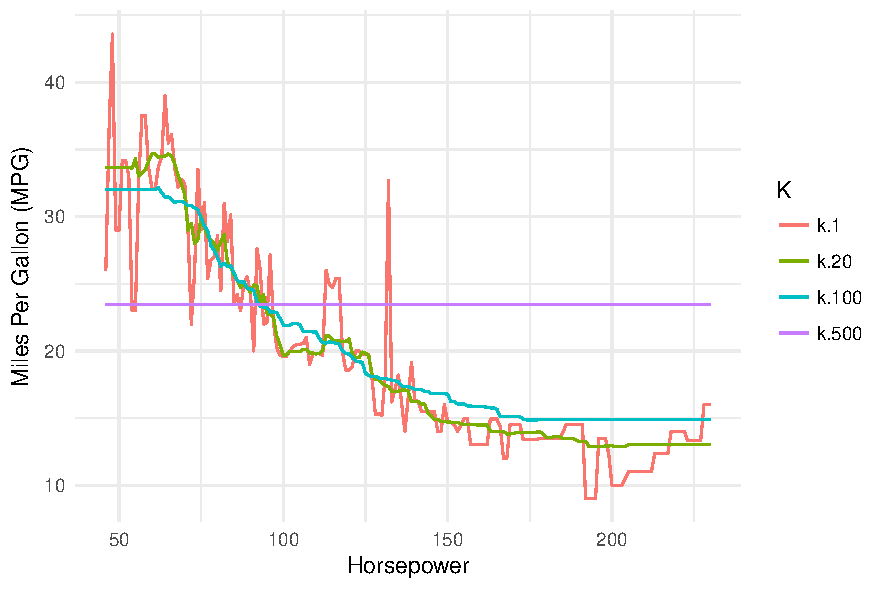
\includegraphics[width=\linewidth]{../figs/class1/auto_knn_compare.pdf}\end{center}
\end{frame}

\begin{frame}\frametitle{Questions ...}
\begin{itemize}
    \item How to choose $k$?
    \item Are there better methods?
\end{itemize}
\end{frame}

\begin{frame} \frametitle{Machine Learning Choices ...}
    \centering
    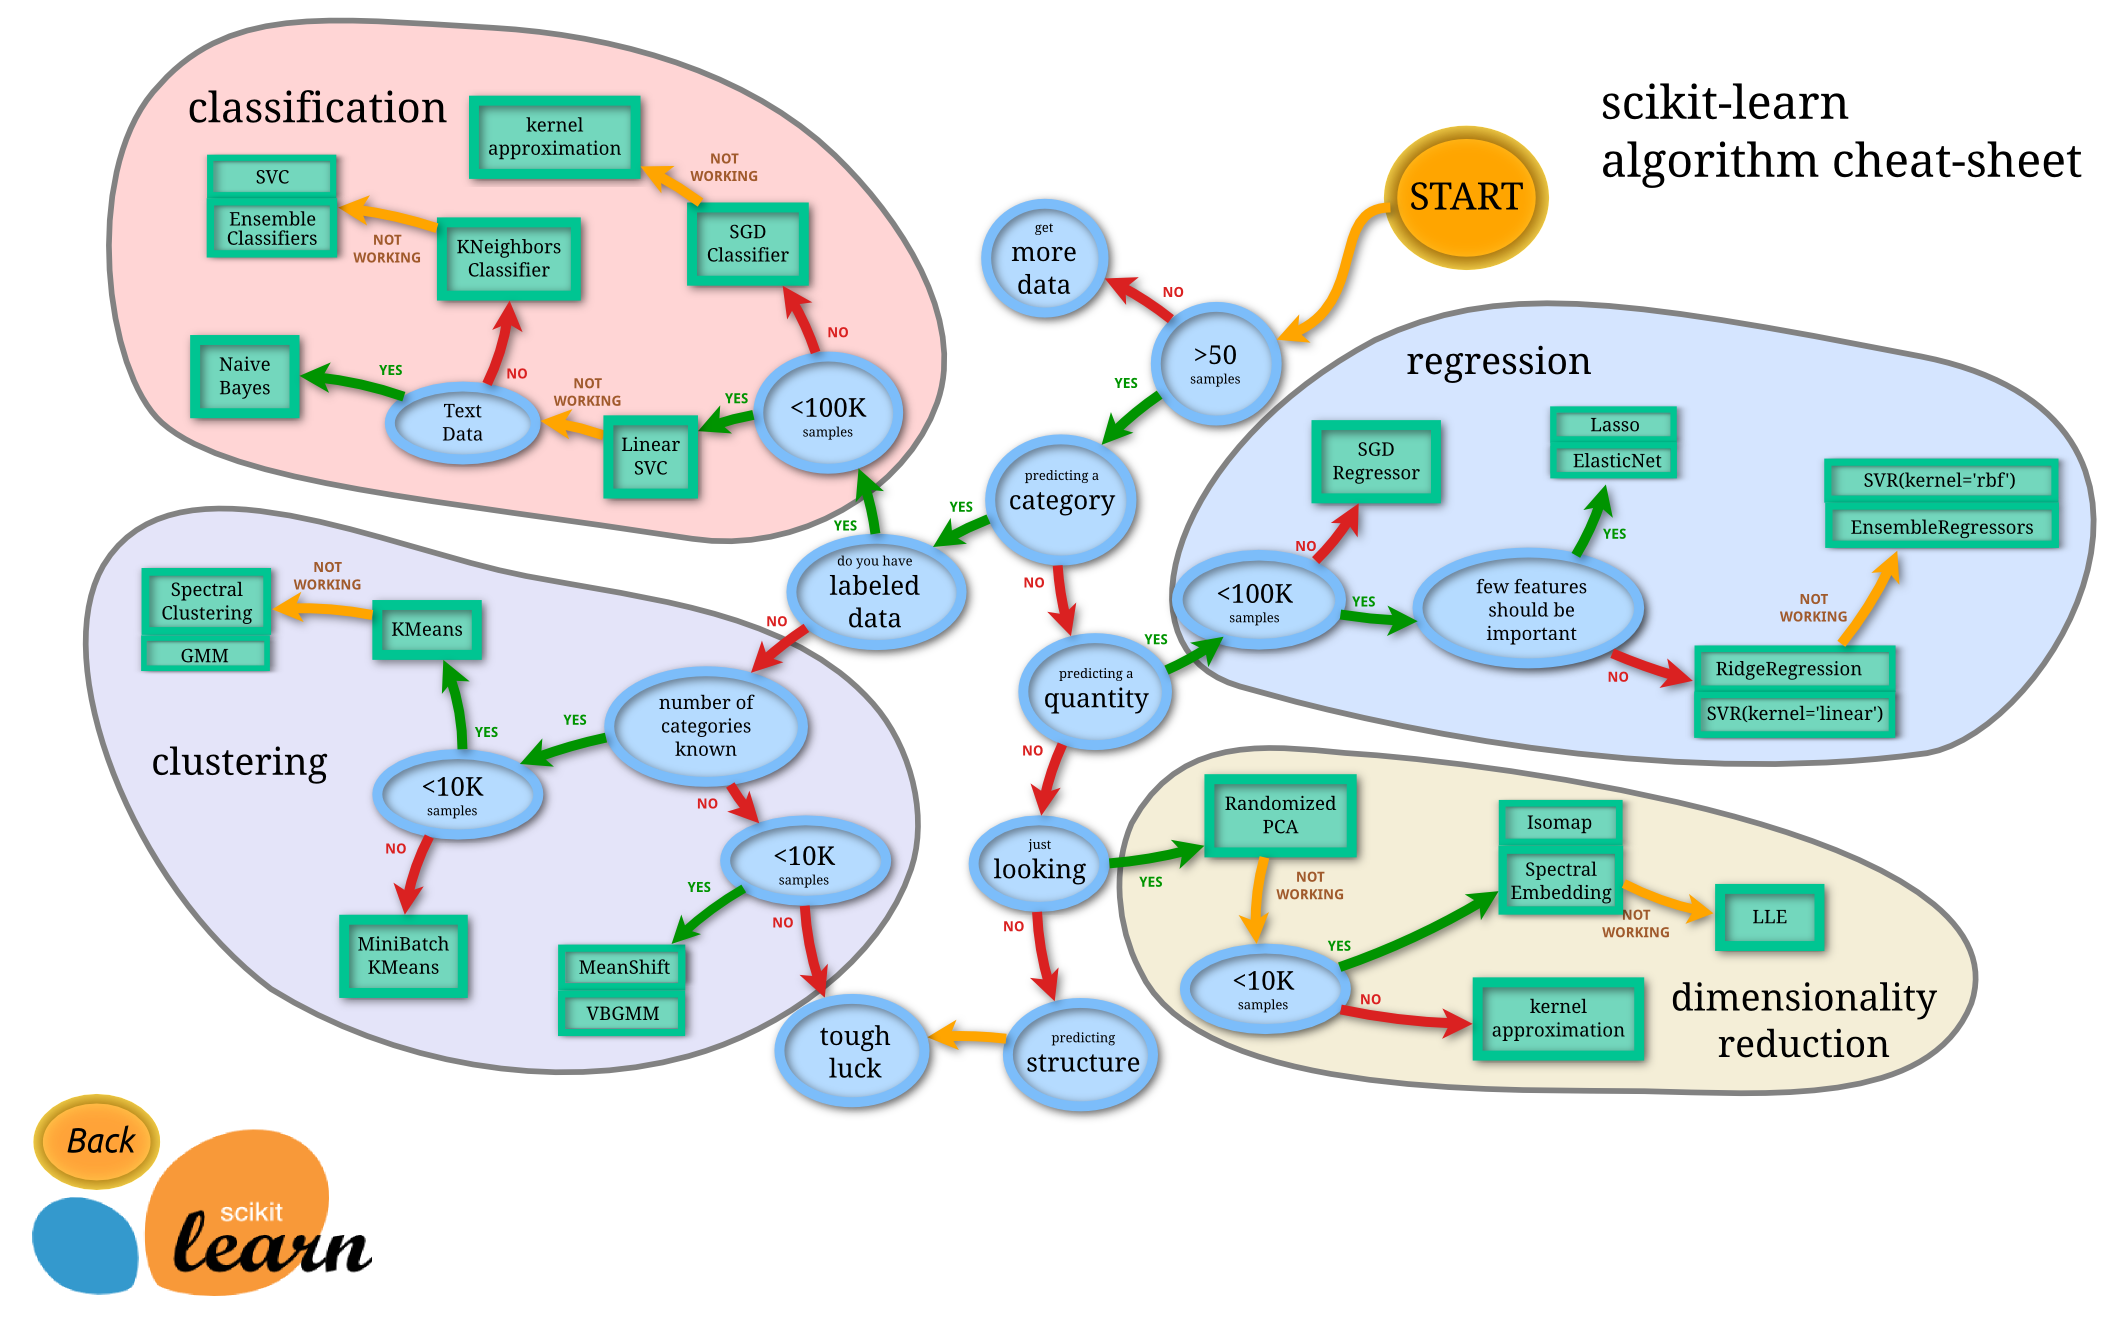
\includegraphics[width=\linewidth]{../figs/class1/ml_map.png}\\
    {\tiny Source: \url{http://scikit-learn.org/stable/tutorial/machine_learning_map/index.html}} \\[3mm]
    \textbf{End of the semester}: Know what, when, and why to use, know how it works
\end{frame}

\begin{frame}\frametitle{This Course: First Steps in Machine Learning}
\begin{enumerate}
\item \textbf{Foundations}: Mathematics necessary to use and understand ML algoirhtms
\vfill
\item \textbf{Algorithms}: Use common ML algorithms
\vfill
\item \textbf{Principles}: Understand when different algorithms are appropriate
  \vfill
\item 
\end{enumerate}
\end{frame}


\begin{frame} \frametitle{Parametric Prediction Methods}
    Linear regression:
    \[ \varname{MPG} = f(\varname{horsepower}) = \beta_0 + \beta_1 \times \varname{horsepower}  \]
    \begin{center}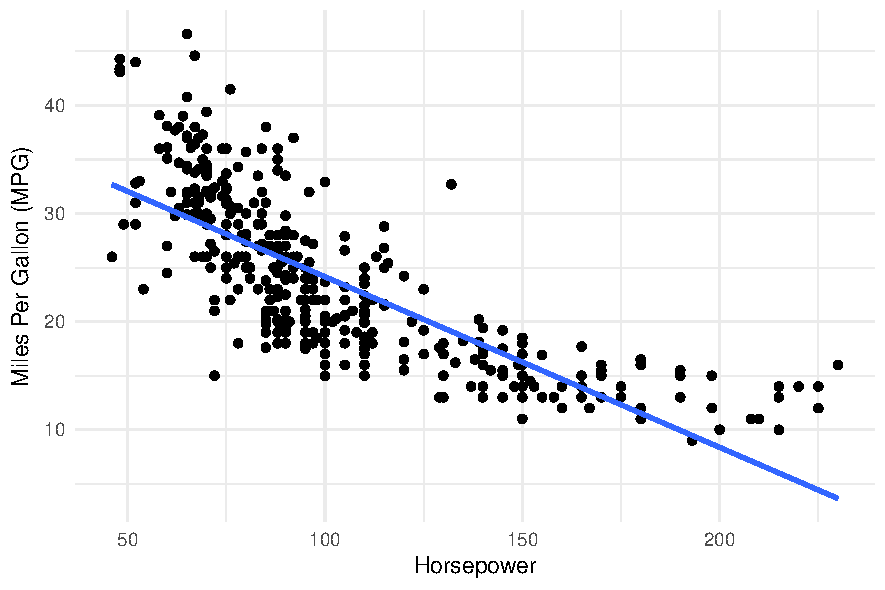
\includegraphics[width=0.8\linewidth]{../figs/class1/auto_data_regression.pdf}
    \end{center}
\end{frame}


\begin{frame} \frametitle{R Language}
\begin{itemize}
\item Download and install R: \url{http://cran.r-project.prg}
\vfill
\item Try using RStudio as an R IDE
\vfill
\item \emph{See class website for more info}
\vfill
\item All my R code is in the class git repo
\vfill
\item You can use Python or another language, but at your own risk
    \end{itemize}
\end{frame}

%\begin{frame} \frametitle{Alternatives to R}
%\begin{itemize}
%\item \textbf{Python} (+ Numpy + Pandas + Matplotlib + Scikits Learn + Scipy) \\
%Popular, simpler language, more hassle
%\vfill
%\item \textbf{MATLAB} \\
%Linear algebra and control focus, but a lot of ML toolkits
%\vfill
%\item \textbf{Julia} \\
%New technical computing language, ``walks like python runs like c'', but least mature
%\end{itemize}
%\end{frame}

\begin{frame}{Why R (vs Python)}
\begin{enumerate}
    \item Language syntax particularly suitable for manipulating tabular data
    \item Better-quality packages at \url{cran.r-project.org} than \url{pypi.org}
    \item Excellent data manipulation and visualization tools: dplyr, ggplot, tidyverse, better than python versions like pandas, matplotlib
    \item R-notebooks more flexible and git-friendly than Jupyter
    \item Shiny: a neat web framework to create simple web data interface
    \item Rcpp: convenient interface with C++
    \item Easier to install and use particularly on Windows/Mac
\end{enumerate}
\end{frame}

\begin{frame}{Why Python (vs R)}
    \begin{enumerate}
\item It is popular
\vfill
            \item Better general programming language, good support for data structures
\vfill
            \item Better support for numerical algebra: numpy, scipy,
\vfill
            \item Much better support for deep learning: tensor flow, keras
\vfill
            \item Clean syntax
    \end{enumerate}
\end{frame}

%\begin{frame}{Why Neither Python or R}
%\begin{enumerate}
%    \item Their native code is very slow
%    \item Flexible but error-prone syntax
%    \end{enumerate}
%    \vfill
%    Is Julia is the future?
%\end{frame}

\begin{frame}\frametitle{Logistics}
\begin{itemize}
\item \textbf{Website}:  (get there through mycourses) \\ {\small\url{https://gitlab.cs.unh.edu/carton/ml-fall2025}}
\item \textbf{Grading}: See website
\item \textbf{Assignments}: posted on myCourses at least a week in advance
\item \textbf{Questions}: myCourses Discussion
\item \textbf{Programming language}: R, Python
\end{itemize}
\end{frame}

\end{document}

%%% Local Variables:
%%% mode: latex
%%% TeX-master: t
%%% End:
